\documentclass[a4paper,uplatex,dvipdfmx]{jsarticle}

% ---Display \subsubsection at the Index
% \setcounter{tocdepth}{3}

% ---Setting about the geometry of the document----
% \usepackage{a4wide}
% \pagestyle{empty}

% ---Physics and Math Packages---
\usepackage{amssymb,amsfonts,amsthm,mathtools}
\usepackage{physics,braket,bm}

% ---underline---
\usepackage{ulem}

% ---cancel---
\usepackage{cancel}

% --- surround the texts or equations
% \usepackage{fancybox,ascmac}

% ---settings of theorem environment---
\usepackage{amsthm}
\theoremstyle{definition}
\newtheorem{dfn}{定義}
\newtheorem{prop}{命題}
\newtheorem{thm}{定理}

% ---settings of proof environment---
\renewcommand{\proofname}{\textbf{証明}}
\renewcommand{\qedsymbol}{$\blacksquare$}

% ---Ignore the Warnings---
\usepackage{silence}
\WarningFilter{latexfont}{Some font shapes,Font shape}
\ExplSyntaxOn
\msg_redirect_name:nnn{hooks}{generic-deprecated}{none}
\ExplSyntaxOff

% ---Insert the figure (If insert the `draft' at the option, the process becomes faster.)---
\usepackage{graphicx}
% \usepackage{subcaption}

% ----Add a link to a text---
\usepackage{url,hyperref}
\usepackage[dvipsnames,svgnames]{xcolor}
\hypersetup{colorlinks=true,citecolor=FireBrick,linkcolor=Navy,urlcolor=purple}
\usepackage{pxjahyper}
% ---refer `texdoc xcolor' at the command line---

% ---Tikz---
% \usepackage{tikz,pgf,pgfplots,circuitikz}
% \pgfplotsset{compat=1.15}
% \usetikzlibrary{intersections,arrows.meta,angles,calc,3d,decorations.pathmorphing}

% ---Add the section number to the equation, figure, and table number---
\makeatletter
   \renewcommand{\theequation}{\thesection.\arabic{equation}}
   \@addtoreset{equation}{section}
   
   \renewcommand{\thefigure}{\thesection.\arabic{figure}}
   \@addtoreset{figure}{section}
   
   \renewcommand{\thetable}{\thesection.\arabic{table}}
   \@addtoreset{table}{section}
\makeatother

% ---enumerate---
% \renewcommand{\labelenumi}{$\arabic{enumi}.$}
% \renewcommand{\labelenumii}{$(\arabic{enumii})$}

% ---Index---
% \usepackage{makeidx}
% \makeindex 

% ---Fonts---
% \renewcommand{\familydefault}{\sfdefault}
% \renewcommand{\kanjifamilydefault}{\gtdefault}

% ---Title---
\title{AdS/CFT対応とエンタングルメントエントロピー}
\author{宮根 一樹}
\date{2023年 12月 21日}

\begin{document}

\maketitle

\tableofcontents

\clearpage
\section{はじめに}

物理学科B4の宮根です.12/21の記事を担当します.

今回の記事では,理論物理学で最近盛んに研究されているAdS/CFT対応について紹介しようと思っています.もともと情報理論ゼミ\footnote{
  「情報理論ゼミ」とは今となっては名ばかりで,情報理論をまじめに勉強していたのはゼミが発足してから数か月くらいでした.それ以降はずっとオムニバス形式をとっており,情報理論に関係あることないこと好き放題話しています(量子情報のときもあれば,関数解析のときもありました).
}で私が何度か話をしてきた内容で,ここではそれらを体系的にまとめてみました.

AdS/CFT対応自体はなかなか高級な理論で,よく知られているのは$d=4$の$\mathcal{N}=4$超対称ヤン=ミルズ理論と$\text{AdS}_{5}\times S_{5}$上での超弦理論との対応でした.これらの理論は結合定数の対応関係という,物理的なパラメターの対応として研究されていたそうです.これらの対応関係は非常に不思議なもので,ヤン=ミルズ理論は\textbf{ゲージ}理論なのに対し,超弦理論は\textbf{量子重力}理論に対応関係があるといっています.

現在の素粒子標準模型は,ゲージ群が$SU(3)\times SU(2)\times U(1)$のヤン=ミルズ理論によって記述されていますが,ゲージ理論を考えている限り,スピンが2である重力子(グラビトン)から物理的な量を取り出すことができません.超弦理論ではこの標準模型が,\textbf{開弦}$+$Dブレーンの低エネルギー有効理論として埋め込まれていると考えられています.一方で,超弦理論では\textbf{閉弦}が重力として入っており,AdS/CFT対応が面白いのは,ゲージ理論と閉弦の理論の間に対応関係があるということです.これはある意味,「重力も何かしらの意味でゲージ理論で書けるのではないか」といった可能性を示唆しています.

と,AdS/CFT対応のゲージ/重力対応的な側面を見てきましたが,その一方で,それぞれの時空のエントロピーも対応していることが示唆されました\cite{Ryu_AspectsHolographic_2006}.本稿では,情報理論ゼミの一環として,そのような時空のエントロピーの対応関係について紹介しようと思います.この記事を読むためには,少し発展的な物理の知識があると楽しめるかもしれません.具体的に言えば,相対性理論や場の量子論,量子情報,そして(物理としての)群論の基礎的な内容でしょう\footnote{
  相対性理論や場の量子論といいましたが,テクニカルなこと(エネルギー・運動量テンソルとか,ファインマンダイアグラムとか)は用いません.相対性理論としては,時空の計量がどのような物理的描像を与えるのか,ということを知っていれば十分ですし,場の量子論としては,経路積分の思想を知っていれば十分でしょう.量子情報については,フォン=ノイマンエントロピーがどんな感じか分かっていれば頭に入ってくるはずです.
}.

とはいえ,私の理解を多めに書くようにしているので,あまり物理が分からない方でもよく楽しんでいただけるのではないでしょうか(実際に,知らない分野のアドカレを眺めていても楽しいときは楽しいですしね).せっかくの企画記事ですので,肩の力を抜いて,私の分野の雰囲気を味わっていただければと思います\footnote{
  そのまま,あいまいな記述があっても目をつむっていただけると...
}.


\clearpage

\section{AdS/CFT対応}

素粒子理論では,場の理論が時空の対称性によって強く規定される.AdS/CFT対応はこの思想に基づいており,時空の構造が違くても,対称性が同じであるのなら,それらの時空で展開される場の理論が等価であることが期待される.この章では,時空の対称性がどのようにして場の理論に関係しているのかをおさらいして,なぜAdS空間とCFT空間の理論の間に対応関係があるのかを見ていく.

\subsection{場の理論と対称性}
\label{symmetry}

私たちが住んでいる時空は相対論的であり,ローレンツ変換に対して不変であることがわかっている.したがって,フォーマルに「ラグランジアン$\rightarrow$運動方程式」と理論を構築していく解析力学的なアプローチをとるなら,そもそものスタートラインであるラグランジアンをローレンツ不変に構成しておくのがよいだろう.今,私たちの時空は$4$次元であるとすると,その世界距離は
\begin{equation}
  \dd s^2
  =
  g_{\mu\nu}\dd x^{\mu}\dd x^{\nu}
  \label{world_dist}
\end{equation}
となっており,時空の構造は軽量テンソル$g_{\mu\nu}$によって決定される.今,簡単にこの時空が平坦
\begin{equation}
  g_{\mu\nu}
  =
  \eta_{\mu\nu}
  =
  \text{diag}(-,+,+,+)
\end{equation}
だとして話を進めてみる.この時空は\textbf{ミンコフスキー空間}と呼ばれる.このとき,この時空に住むベクトルは$A^{\mu}=(A^{0},\bm{A})$と書くことができ,``内積''$A^{\mu}A_{\mu}$が定義される\footnote{
  ``内積''としたのは,本当は内積ではないからである.非退化性や半正定値性とか.
}.世界距離\eqref{world_dist}もこの内積を用いて$\dd s^2=\dd x^{\mu}\dd x_{\mu}$と書くことができる.

一般に「対称性」といった場合は,この内積を保つような変換のことを意味する.そのような変換を\textbf{ローレンツ変換}という.実ベクトルの内積を保つような変換は直交群をなすが,ミンコフスキー空間の内積は少し特殊で
\begin{equation}
  \dd s^2
  =
  -(\dd {x^{0}})^2
  +(\dd {x^{1}})^2
  +(\dd {x^{2}})^2
  +(\dd {x^{3}})^2
\end{equation}
なので,このローレンツ変換がなす群を\textbf{ローレンツ群}といい,先ほどのような事情から$SO(3,1)$と書くことにして直交群とは区別する\footnote{
  内積を保つだけなら$O(3,1)$でもよいが,$\det\Lambda=1$のものをとってくることにする.
}.

今度は,このローレンツ群$SO(3,1)$の\textbf{表現}を考えよう\footnote{
  どうやら,数学的に正しいのは「表現から誘導される微分表現」らしい.詳しいことは知りません.このことは九後先生の教科書\cite{九後_ゲー_1989a}の脚注に記述があった.
}.ここでいう表現とは,$\Lambda\in SO(3,1)$を行列に対応させる写像$D$のことをいう.ただし,$D$は(思いつく限り)
\begin{itemize}
  \item 
  恒等変換$e\in SO(3,1)$は,単位行列$D(e)=I$になる.
  \item 
  変換を連続に行ったもの$\Lambda_{1}\cdot\Lambda_{2}$は,行列の積$D(\Lambda_{1})\cdot D(\Lambda_{2})$になる.
\end{itemize}
などの性質を満たす.

ローレンツ群$SO(3,1)$の生成子は,角運動量の生成子$J_{i}$と並進の生成子$K_{i}$の6つであることが知られている.それらは
\begin{equation}
  \left\{
    \begin{alignedat}{1}
      [J_{i},J_{j}]
      =
      i\varepsilon_{ijk}J_{k}
      ,
      \\
      [J_{i},K_{j}]
      =
      i\varepsilon_{ijk}K_{k}
      ,
      \\
      [K_{i},K_{j}]
      =
      -i\varepsilon_{ijk}J_{k}
    \end{alignedat}
  \right.
  \label{gene_angl_bos}
\end{equation}
を満たしており,これらはローレンツ変換$\Lambda\in SO(3,1)$とは
\begin{gather}
  M^{ij}
  \equiv
  \varepsilon^{ijk}J_{k}
  ,\quad
  M^{i0}
  \equiv
  K_{i}
  \\
  \Lambda
  =
  \exp
  \left(  
    -\frac{i}{2}\varepsilon^{\mu\nu}M_{\mu\nu}
  \right)
\end{gather}
と結びついている.表現を考えたとき,これらの関係式はすべて保たれることになる.

さて,\eqref{gene_angl_bos}に対して,
\begin{equation}
  A^{i}
  \equiv
  \frac{1}{2}(J^{i}+iK^{i})
  ,\quad
  B^{i}
  \equiv
  \frac{1}{2}(J^{i}-iK^{i})
\end{equation}
と$A^{i},B^{i}$を定義すれば
\begin{equation}
  \left\{
    \begin{alignedat}{1}
      [A_{i},A_{j}]
      &=
      i\varepsilon_{ijk}A_{k}
      ,
      \\
      [B_{i},B_{j}]
      &=
      i\varepsilon_{ijk}B_{k}
      ,
      \\
      [A_{i},B_{j}]&=0
    \end{alignedat}
  \right.
  \label{gen_AB}
\end{equation}
という交換関係を満たしていることが分かる.この$A_{i},B_{i}$が満たしている交換関係は,$SU(2)$の生成子の交換関係,すなわち角運動量演算子の満たす代数と同じである.

ここで,表現$D(\Lambda)$の行列の大きさを\textbf{表現空間の次元}ということにする\footnote{
  あまり数学的な言い方が分からなかった.下手なことを述べると混乱させると思うので,数学屋はこのような言い回しから察してほしい.
}.この次元とは,物理屋で言うところの角運動量の最大値である.このような事情から
\begin{equation}
  A,B
  =
  0
  ,\ 
  \frac{1}{2}
  ,\ 
  1
  ,\ 
  \frac{3}{2}
  ,\ 
  2
  ,\ 
  \cdots
\end{equation}
と$A,B$は整数か半整数だとすれば,表現の次元は$(2A+1)\times(2B+1)$である.$A_{3},B_{3}$の固有値を$a,b$とすれば,$a=-A,-A+1,\cdots A-1,A$,$b=-B,-B+1,\cdots B-1,B$をとりうる.これらの表現に対応する場を$\varphi_{a,b}(x)$とすれば,考えうる場を全て構成できたことになる\footnote{
  例えば,表現の次元が$(A,B)=(0,0)$の場合はスカラー場であり,それは自明だろう.次は$(A,B)=(1/2,0),(0,1/2)$であり,このときはスピノール場に対応する.
}.



\subsection{反ド・ジッター空間(AdS)と共形場(CFT)}

前節では,場の理論が時空の対称性の表現から記述できることを見てきた.ここでは,そのような観点からAdS/CFT対応が自然と予言されることを見ていこうと思う.

まずは,$(d+2)$次元の反ド・ジッター空間$(\text{AdS}_{d+2})$の対称性について見ていこう.この時空は
\begin{equation}
  \dd s_{d+2}^2
  =
  -
  \dd x_{0}^{2}
  +
  \sum_{i=1}^{d}
  \dd x_{i}^{2}
  -
  \dd x_{d+1}^{2}
\end{equation}
という計量で書かれているため,
\begin{equation}
  g_{\mu\nu}
  =
  \text{diag}
  (-,+,\cdots,+,-)
\end{equation}
である.したがって,$\text{AdS}_{d+2}$の内積を保つ対称性は$SO(d,2)$である.

次に,$(d+1)$次元の共形場$(\text{CFT}_{d+1})$の対称性について考えてみよう.共形場とは,時空$\mathcal{R}^{d,1}$の計量
\begin{equation}
  \dd s_{d+1}^2
  =
  g_{\mu\nu}(x)\dd x^{\mu}\dd x^{\nu}
  \quad
  (\mu,\nu=0,1,\cdots,d)
\end{equation}
が定数倍しか変化しない,すなわち
\begin{equation}
  g(x)
  \rightarrow
  \Omega(x)g_{\mu\nu}
  \label{comf_tf}
\end{equation}
という性質を満たすような変換のことをいう(図\ref{cft_img}).このような変換の生成子を調べ,それらの交換関係について知りたい.そのために,ここでは時空の次元は$d$次元であるとする.

\begin{figure}[ht]
  \centering
  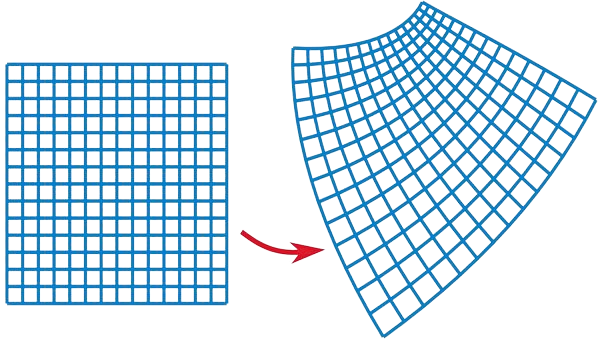
\includegraphics[keepaspectratio,width=0.8\linewidth]{fig/cft_img.png}
  \caption{共形変換のイメージ.\underline{各点の}形(角度とか)が保たれている.}
  \label{cft_img}
\end{figure}

生成子とは,無限小変換に対応しているとみなせるため\footnote{
  今回は省略したが,ローレンツ群の生成子も同様に無限小変換を考えることによって導出する.
},$x^{\mu}\rightarrow x^{\mu}+\varepsilon^{\mu}(x)$と無限小のベクトル$\varepsilon^{\mu}$だけずらしたとしてみよう.この変換は,座標に依存するローカルな変換であることに注意すれば
\begin{align}
  \dd s_{d+1}^2
  &=
  \eta_{\mu\nu}
  \dd x^{\mu}\dd x^{\nu}
  \nonumber
  \\
  &\rightarrow
  (\dd x_{\mu}+\partial_{\nu}\varepsilon_{\mu}\dd x^{\nu})
  (\dd x^{\mu}+\partial_{\nu}\varepsilon^{\mu}\dd x^{\nu})
  \nonumber
  \\
  &\sim
  \left( \eta_{\mu\nu}+\partial_{\mu}\varepsilon_{\nu}+\partial_{\nu}\varepsilon_{\mu} \right)
  \dd x^{\mu}\dd x^{\nu}
\end{align}
となるので,計量は
\begin{equation}
  \eta_{\mu\nu}
  \rightarrow
  \eta_{\mu\nu}
  +
  \partial_{\mu}\varepsilon_{\nu}+\partial_{\nu}\varepsilon_{\mu}
\end{equation}
と変化したことになる.\eqref{comf_tf}と照らし合わせると,ある関数$\sigma(x)$に対して
\begin{equation}
  \partial_{\mu}\varepsilon_{\nu}+\partial_{\nu}\varepsilon_{\mu}
  =
  2\sigma(x)\eta_{\mu\nu}  
  \label{sec2_2_eq1}
\end{equation}
という関係式を$\varepsilon_{\mu}$は満たしていなければならないことが分かる.なお,ここで$\sigma(x)$は微小量であり,\eqref{comf_tf}の$\Omega(x)$に対して
\begin{equation}
  \Omega(x)
  =
  1+2\sigma(x)+\mathcal{O}(\sigma^2)
\end{equation}
としている.\eqref{sec2_2_eq1}より$\partial_{\mu}\varepsilon^{\mu}=d\cdot \sigma(x)$であり,さらに$\eta^{\mu\nu}\eta_{\mu\nu}=d-2$であることに注意すれば
\begin{equation}
  (\eta_{\mu\nu}\partial^{2}-(d-2)\partial_{\mu}\partial_{\nu})\partial\cdot\varepsilon
  =
  0
  \label{sec2_2_eq2}
\end{equation}
が成立していることが分かる.この等式\eqref{sec2_2_eq2}を見れば分かる通り,共形変換は$d=2$では特異的である.

ここでは,次元は$d>2$だとしておこう.このときは,\eqref{sec2_2_eq2}を満たすような無限小変換$\varepsilon^{\mu}$を見つければよい.そのような変換は$x$の2次までで
\begin{equation}
  \varepsilon^{\mu}(x)
  =
  a^{\mu}
  +
  \omega^{\mu}_{\ \nu}x^{\nu}
  +
  \lambda x^{\mu}
  +
  b^{\mu}x^2
  -
  2(b\cdot x)x^{\mu}
\end{equation}
となっている(任意の次元d($d>2$)で成立するためには,3次以上はない).ここで,$a^{\mu}, \omega^{\mu}_{\ \nu}, \lambda, b^{\mu}$は無限小パラメターであり,それぞれ並進,ローレンツ変換,ディラテーション,特殊共形変換を生成している.それぞれの生成子を$P_{\mu},\ J_{\mu\nu},\ D,\ K_{\mu}$と書くことにすると,これらの生成子の交換関係は
\begin{equation}
  \left\{
    \begin{alignedat}{1}
      [J_{\mu\nu},K_{\rho}]
      &=
      i(\eta_{\mu\rho}K_{\nu}-\eta_{\nu\rho}K_{\mu})
      ,
      \\
      [D,P_{\mu}]
      &=
      iP_{\mu}
      ,\ 
      [D,K_{\mu}]
      -
      -iK_{\mu}
      ,\ 
      [D,J_{\mu\nu}]
      =
      0
      ,
      \\
      [K_{\mu},K_{\rho}]
      &=
      0
      ,\ 
      [K_{\mu},P_{\nu}]
      =
      -2i(\eta_{\mu\nu}D-J_{\mu\nu})
    \end{alignedat}
  \right.
  \label{comf_generator}
\end{equation}
を満たしている\footnote{
  この関係を示すためには,これらの生成子が
  \begin{equation}
    a^{\mu}\partial_{\mu},\ 
    \omega^{\mu}_{\ \nu}\varepsilon^{\mu}\partial_{\mu},\ 
    \lambda x\cdot\partial,\ 
    b^{\mu}(x^2 \partial_{\mu}-2x^{\mu}x\cdot\partial)
    \nonumber
  \end{equation}
  と書けることを用いればよい.
}.

実は,交換関係\eqref{comf_tf}は$SO(d,2)$の代数と(局所的に)同型であることが分かっており,これは,$\text{AdS}_{d+2}$の対称性と一致している\footnote{
  $SO(d,2)$の生成子をうまく取り直すと,\eqref{comf_generator}が再現されます.例えば,\cite{Ammon_GaugeGravity_2015}を参照.
}.「対称性が一致しているから理論は同じ」というわけにはいかないが,このことがAdS/CFT対応の1つのモチベーションなのだろう.


\subsection{AdS空間の幾何}

この章の終わりとして,少しAdS空間の幾何学的な側面を見ていこうと思う(ここでいう幾何というのは,曲面論的な話).なお,今回は重力理論的な側面を中心に紹介しようと思うが,物性的な側面や数理物理的な側面が気になる方はSGCライブラリの佐藤先生の本\cite{佐藤_弦理_2021}を読んでみるとよいかもしれない.

AdS空間の計量を再び書いておくと
\begin{equation}
  \dd s^2
  =
  -\dd X_{0}^{2}
  +
  \sum_{i=1}^{d}
  \dd X_{i}^{2}
  -
  \dd X_{d+1}^2
\end{equation}
である.この時空の境界面のうち
\begin{equation}
  -X_{0}^{2}
  +
  \sum_{i=1}^{d}
  X_{i}^{2}
  -
  X_{d+1}^2
  =
  0
  \label{comf_boundary}
\end{equation}
であるようなものは,共形変換で不変な境界である.AdS計量とミンコフスキー計量と結びつけ,このような境界がミンコフスキー時空でどのようにして現れてくるのかを調べたい.ここでは,次の座標変換
\begin{equation}
  \left\{
    \begin{alignedat}{1}
      X_{0}
      &=
      \frac{L^2}{2r}
      \left(  
        1
        +
        \frac{r^2}{L^4}(\bm{x}^2-x_{0}^{2}+L^2)
      \right)
      ,
      \\
      X_{i}
      &=
      \frac{r}{L}x_{i}
      ,
      \\
      X_{d}
      &=
      \frac{L^2}{2r}
      \left(  
        1+\frac{r^2}{L^4}(\bm{x}^2-x_{0}^2-L^2)
      \right)
      ,
      \\
      X_{d+1}
      &=
      \frac{r}{L}x_{0}
    \end{alignedat}
  \right.
\end{equation}
をしてみよう(ポアンカレパッチ).ここで,$L$は正のパラメターである.少し天下りな変換のように見えるが,この変換をすると計量は
\begin{equation}
  \dd s^2
  =
  \frac{L^2}{r^2}\dd r^2
  +
  \frac{r^2}{L^2}(-\dd t^2+\dd \bm{x}^2)
\end{equation}
と書ける.第2項を見れば分かる通り,ある$r$を固定してしまえば,この時空はミンコフスキーとなっており\footnote{
  この時空の真空のアインシュタイン方程式を成立させるためには,宇宙定数が
  $$
    \Lambda
    =
    -
    \frac{d(d-1)}{2L^2}
    \ 
    (< 0)
  $$
  でなくてはならない.
},それに$r$方向の曲がった方向が付け加えられている.ポアンカレパッチでは共形境界\eqref{comf_boundary}は,$r\rightarrow\infty$で実現されている.本稿で用いるのは,さらに$z=L^2/r$とした座標で
\begin{equation}
  \dd s^2
  =
  \frac{L^2}{z^2}(-\dd t^2+\dd z^2+\dd x^2)
  \label{AdS_metric_tzx}
\end{equation}
であり,この場合は共形境界が$z=0$に存在することになる.


\section{\texorpdfstring{$(1+1)$}{(1+1)}次元CFTでのエンタングルメントエントロピー}

ここでは,AdS/CFT対応の1つの例として,エントロピーの対応を見ていこうと思う.それぞれの空間のエントロピーは,別々の理論で記述されるが,それらの値が(発散を取り除く操作が入ることがあるが)一致するのは非常にミステリアスである.

この章では,2次元のCFTでの場の理論のエントロピーの計算を行う.特に,空間上にあるインターバル$[u,v]$があるとして,そのような真空のエントロピーを計算する\footnote{
  ちなみに``インターバルがある''といったが,これが物理的にどのような意味を持っているかは恥ずかしながら私はよく分かっていない.
}.次章では,ここで求めたエントロピーがAdS空間上でもうまく取り扱えることを見ていく.

\subsection{エンタングルメントエントロピー}

量子力学についての理解が進むにつれて,熱力学的な量を量子論の立場から解釈できるようになった.量子論におけるエントロピーの1つの形式は,密度行列$\rho$に対して定義される\textbf{フォンノイマンエントロピー}
\begin{equation}
  S
  \equiv
  -\text{tr}\rho\log\rho  
\end{equation}
である.フォンノイマンエントロピーは,密度行列$\rho$が対角化されているとすれば,形式的にシャノンエントロピーと一致しており,このフォンノイマンエントロピーを考えるのは有用だと考えることができる.しかしながら,より実践的な立場となると,フォンノイマンエントロピーを計算するのが大変な場合がある.今回,これから計算することもそのようなケースである.そこで,次の\textbf{レニーエントロピー}
\begin{equation}
  S_{n}
  \equiv
  \dfrac{1}{1-n}\log\text{tr}_{A}\rho_{A}^{n}
  \label{renyi_E}
\end{equation}
を考えることにしよう.ここでは,$A$は時空のある領域を考えることにしている(後述).レニーエントロピーの極限
\begin{equation}  
  S_{n}
  \rightarrow
  S
  \quad
  (n\rightarrow 1)
\end{equation}
はフォンノイマンエントロピーを与える\footnote{
  証明は少しめんどくさい.気になった方は,\cite{Muller-Lennert_QuantumRenyi_2013}などを参考にしてトライするとよいだろう.先ほどの文献が重いならなら,\href{https://physics.stackexchange.com/questions/73424}{これとか}も参考になる.
  \label{note_renyi}
}\footnote{
  今回はフォンノイマンエントロピーをレニーエントロピーの極限として定義するフォーマリズムをとったが,この他にもツァリスエントロピーというのを用いて計算する方法もある.オリジナルがそのような定式化をしていた.
}ので,この性質を利用すると,エントロピーを計算できる場合がある.


\subsection{レプリカ法}

場の理論でエントロピーを計算することを考えよう.ここでは,時空は$(1+1)$次元のCFTとし,領域$A$は$A=\{(t_{E},x)\in\mathbb{R}^2|t_{E}=0,x\in[u,v]\}$とする.なお,$t_E$はウィック回転後の座標で,元の座標に対して$t_E=it$と定義されているものとする.\eqref{renyi_E}の表式を見ると,$\tr_{A}\rho_{A}^{n}$を求めることができればエントロピーが計算できるように思える.$\rho_{A}^{n}$を計算するのは大変なようにみえるが,場の量子論における経路積分と,CFTで知られているツイスト場による構成を行えば,この計算を直観的に遂行することができる.

まずは,密度行列を定義しておこう.量子力学においては,波動関数の状態$\ket{\psi}$を用いれば
\begin{equation}
  \rho
  =
  \ketbra{\psi}{\psi}
\end{equation}
と書けたので,密度行列の$(i,j)$成分が
\begin{equation}
  (\rho)_{ij}
  =
  \ev*{i|\psi}\ev*{\psi|j}
  =
  \psi_{i}\bar{\psi}_{j}
\end{equation}
のように形式的に書けることを,場の理論に拡張していく.場の理論における基底は場の演算子$\phi$に対する基底$\ket{\phi}$を一般に用いることにすれば,$(\phi_1,\phi_2)$のように,密度行列の成分は場をとることになるだろう.つまり,(未定義ではありますが)波動関数$\Psi[\phi]$を用いて
\begin{equation}
  (\rho)_{\phi_1\phi_2}
  \equiv
  \Psi[\phi_1]\bar{\Psi}[\phi_2]
\end{equation}
と定義しておくのがよさそうである.しかし,ここで欲しいのは部分領域$A$における密度行列であることに注意しよう.したがって,波動関数の変数となるべき場は$(t_E,x)\in[u,v]$で定義されているべきで
\begin{equation}
  (\rho_{A})_{\phi^{A}_{1}\phi^{A}_{2}}
  \equiv
  \Psi[\phi^{A}_1]\bar{\Psi}[\phi^{A}_2]
  \label{density_matrix_A}
\end{equation}
である.

さて,次に波動関数を定義しよう.量子力学における波動関数は,経路積分の形で書くと
\begin{equation}
  \psi(t_{E},x)
  =
  \ev*{x|e^{-iHt_{E}}|x_i}
  =
  \int
  \mathcal{D}x\ 
  e^{-S[x]}
\end{equation}
であった.ここで,$x^{i}$は任意の基準点である.このことから,場の理論での波動関数は
\begin{equation}
  \Psi[\phi^{A}]
  \equiv
  \int_{\phi(-\infty,x)=\phi'(x)}^{\phi(-0,x)=\phi^{A}(x)}\mathcal{D}\phi\ 
  e^{-S[\phi]}
\end{equation}
と定義することができるだろう.この経路積分の意味だが,「$t_{E}=-\infty$の時間での場が$\phi'(x)$だったとして,そこから$t_E=0$までの寄与をすべて足し上げる」といった感じになっている.$\phi'(x)$は量子力学の場合の基準点なので,ここでは任意である.この複素共役$\bar{\Psi}[\phi^{A}]$は,これまた量子力学の場合
\begin{equation}
  \psi^{*}(t_{E},x)
  =
  \ev*{x_i|e^{-iH(-t_{E})}|x}
  =
  \int
  \mathcal{D}x\ 
  e^{-S[x]}
\end{equation}
を参考にすれば
\begin{equation}
  \bar{\Psi}[\phi^{A}]
  \equiv
  \int_{\phi(+0,x)=\phi^{A}(x)}^{\phi(+\infty,x)=\phi'(x)}\mathcal{D}\phi\ 
  e^{-S[\phi]}
\end{equation}
となるはずである.このことから,密度行列\eqref{density_matrix_A}は
\begin{equation}
  (\rho_{A})_{\phi^{A}_{-}\phi^{A}_{+}}
  =
  \int_{\phi(-\infty,x)=\phi'(x)}^{\phi(-0,x)=\phi_{-}^{A}(x)}\mathcal{D}\phi\ 
  e^{-S[\phi]}
  \cdot
  \int_{\phi(+0,x)=\phi_{+}^{A}(x)}^{\phi(+\infty,x)=\phi'(x)}\mathcal{D}\phi\ 
  e^{-S[\phi]}
  \label{dens1}
\end{equation}
となる.これを少し計算すると
\begin{equation}
  (\rho_{A})_{\phi^{A}_{-}\phi^{A}_{+}}
  =
  \frac{1}{Z_1}
  \int_{A}\mathcal{D}\phi\ 
  e^{-S[\phi]}
  ,\quad
  Z_{1}
  =
  \int\mathcal{D}\phi\ 
  e^{-S[\phi]}
\end{equation}
と書くことができる\footnote{
  経路積分の離散化を思い出してみると,測度$\mathcal{D}$のほうは$N$回(最後に$N\rightarrow\infty$とするが)の積分に書き換えられることから,
  $$
    \int_{A}\mathcal{D}\phi
    \int_{B}\mathcal{D}\phi
    =
    \int_{A+B}\mathcal{D}\phi
  $$
  といったことが経路積分では成り立つと考えることができる.これは,普通の積分とは異なるので少し注意が必要である.
  \label{footnote_path}
}.ただし,「領域$A$での経路積分」は
\begin{equation}  
  \int_{A}\mathcal{D}\phi
  \equiv
  \int\mathcal{D}\phi\ 
  \prod_{x\in A}
  \delta(\phi(-0,x)-\phi_{-}(x))
  \delta(\phi(+0,x)-\phi_{+}(x))
  \label{path_int_A}
\end{equation}
の意味であり,「$x\in A$のとき,$t_{E}=+0$と$t_{E}=-0$の寄与を別々に拾ってくる」という意味になる.なお,このデルタ関数が働くのは$x\in A$のときのみであり,$x\notin A$のときは値を1とみなしている.普通のデルタ関数の意味とは違うので注意が必要である\footnote{
  $A$上では境界条件$t_{E}=-0$では$\phi(-0,x)=\phi_{-}(x)$,$t_{E}=+0$では$\phi(+0,x)=\phi_{+}(x)$が効いてきて,他のところは普通の経路積分で寄与を拾ってきている.
}.また,$Z_1$は規格化$\tr_{A}\rho_{A}=1$するための因子である.(この意味はすぐわかる)

\begin{figure}[ht]
  \centering
  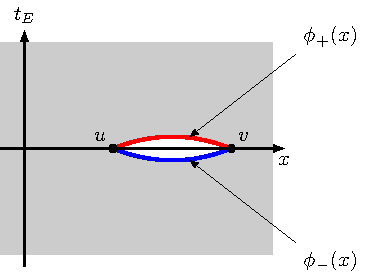
\includegraphics[keepaspectratio]{fig/path_int_region/path_int_region.pdf}  
  \caption{経路積分\eqref{path_int_A}の概略}
  \label{path_int_region}
\end{figure}

密度行列が定義できたので,今度は$\tr_{A}\rho_{A}^n$の計算に移ろう.量子力学をまたも足掛かりにすれば,トレースは
\begin{equation}
  \tr_{A}\rho_{A}^{n}
  =
  \int_{A}\mathcal{D}\phi_{1}\ 
  (\rho_{A}^{n})_{\phi_{1}\phi_{1}}
  \label{dens2}
\end{equation}
となる.また積は$(\rho^2)_{ij}=\sum\rho_{ik}\rho_{kj}$となっていたことから,場の理論では
\begin{equation}
  (\rho_{A}^{n})_{\phi_{1}\phi_{1}}
  =
  \int_{A}\mathcal{D}{\phi_{2}}
  \cdots
  \int_{A}\mathcal{D}{\phi_{n}}\ 
  (\rho_A)_{\phi_{1}\phi_{2}}
  \cdots
  (\rho_A)_{\phi_{n}\phi_{1}}
\end{equation}
である.これを\eqref{dens2}に代入すれば
\begin{equation}
  \tr_{A}\rho_{A}^{n}
  =
  \int_{A}\mathcal{D}\phi_{1}
  \cdots
  \int_A\mathcal{D}{\phi_{n}}\ 
  (\rho_A)_{\phi_{1}\phi_{2}}
  \cdots
  (\rho_A)_{\phi_{n}\phi_{1}}
  \label{dens3}
\end{equation}
という表式を得る.この積分は$\mathbb{R}^2$の上を$\phi_1,\cdots,\phi_n$で積分しているとみなせるが,ここでは「$\mathbb{R}^2$が$n$枚あって,それぞれのシートの上で経路積分をし,デルタ関数の部分で境界をつなげている」という見方をしてみる.

いきなり$n$枚のケースを考えるのは大変なので,$n=2$の場合を考えてみよう.$n=2$のときは
\begin{align}
  \int_{A}\mathcal{D}\phi_1\ 
  (\rho_{A}^2)_{\phi_1\phi_1}
  &=  
  \int_{A}\mathcal{D}\phi_1
  \int_{A}\mathcal{D}\phi_2\ 
  (\rho_{A})_{\phi_1\phi_2}(\rho_{A})_{\phi_2\phi_1}
  \nonumber
  \\
  &=
  \frac{1}{Z_{1}^2}
  \int_{A}\mathcal{D}\phi_1
  \int_{A}\mathcal{D}\phi_2
  \int\mathcal{D}\phi^{\prime}
  \ 
  e^{-S[\phi^{\prime}]}
  \int\mathcal{D}\phi^{\prime\prime}
  \ 
  e^{-S[\phi^{\prime\prime}]}
  \nonumber
  \\
  &\qquad\times
  \prod_{x\in A^{\prime}}
  \uwave{\delta(\phi^{\prime}(-0,x)-\phi_1(x))}\delta(\phi^{\prime}(+0,x)-\phi_2(x))
  \nonumber
  \\
  &\qquad\times  
  \prod_{x\in A^{\prime\prime}}
  \delta(\phi^{\prime\prime}(-0,x)-\phi_2(x))\uwave{\delta(\phi^{\prime\prime}(+0,x)-\phi_1(x))}
\end{align}
となるが,デルタ関数の中の場の引数に気をつけて$\phi_1$と$\phi_2$の積分を考えれば,1枚目のシートの$t_{E}=-0$と2枚目のシートの$t_{E}=+0$の場を同一視できることが分かる(もう一方も同様).そのような同一視をいれた2枚の面はリーマン面をなすので,まとめて$\mathcal{R}^{n}$と書くことにすれば$n=2$のときは
\begin{equation}
  \tr_{A}\rho_A^2
  =
  \frac{1}{Z_1^2}
  \int_{\mathcal{R}^2}\mathcal{D}\phi\ 
  e^{-S[\phi]}
\end{equation}
とリーマン面$\mathcal{R}^2$での経路積分とみなすことができる\footnote{
  これまでの記法でexplicitに書くと
  $$
    \int_{\mathcal{R}^2}\mathcal{D}\phi
    =
    \int_{\mathbb{R}^2_{(1)}}\mathcal{D}\phi^{\prime}
    \int_{\mathbb{R}^2_{(2)}}\mathcal{D}\phi^{\prime\prime}
    \quad 
    (
      \text{with}
      \quad
      \phi^{\prime}(-0,x)=\phi^{\prime\prime}(+0,x)\ \&\ \phi^{\prime\prime}(-0,x)=\phi^{\prime}(+0,x)
    )
  $$
  といった感じである.$\mathbb{R}^2_{(i)}$とは,$i$枚目の時空であることを表す.
}.あとは,$n=2$の場合を一般化すれば,\eqref{dens3}は
\begin{equation}
  \tr_{A}\rho_{A}^{n}
  =
  \frac{1}{Z_1^n}
  \int_{\mathcal{R}^{n}}\mathcal{D}\phi\ 
  e^{-S[\phi]}
  \equiv
  \frac{Z_n}{Z_1^{n}}
  \label{sec3_1_eq1}
\end{equation}
となり,$\mathcal{R}^n$上での経路積分だと考えることができる.あとは,この空間の分配関数
\begin{equation}
  Z_n
  =
  \int_{\mathcal{R}^{n}}\mathcal{D}\phi\ 
  e^{-S[\phi]}
\end{equation}
を行えばよい.

\begin{figure}[ht]
  \centering
  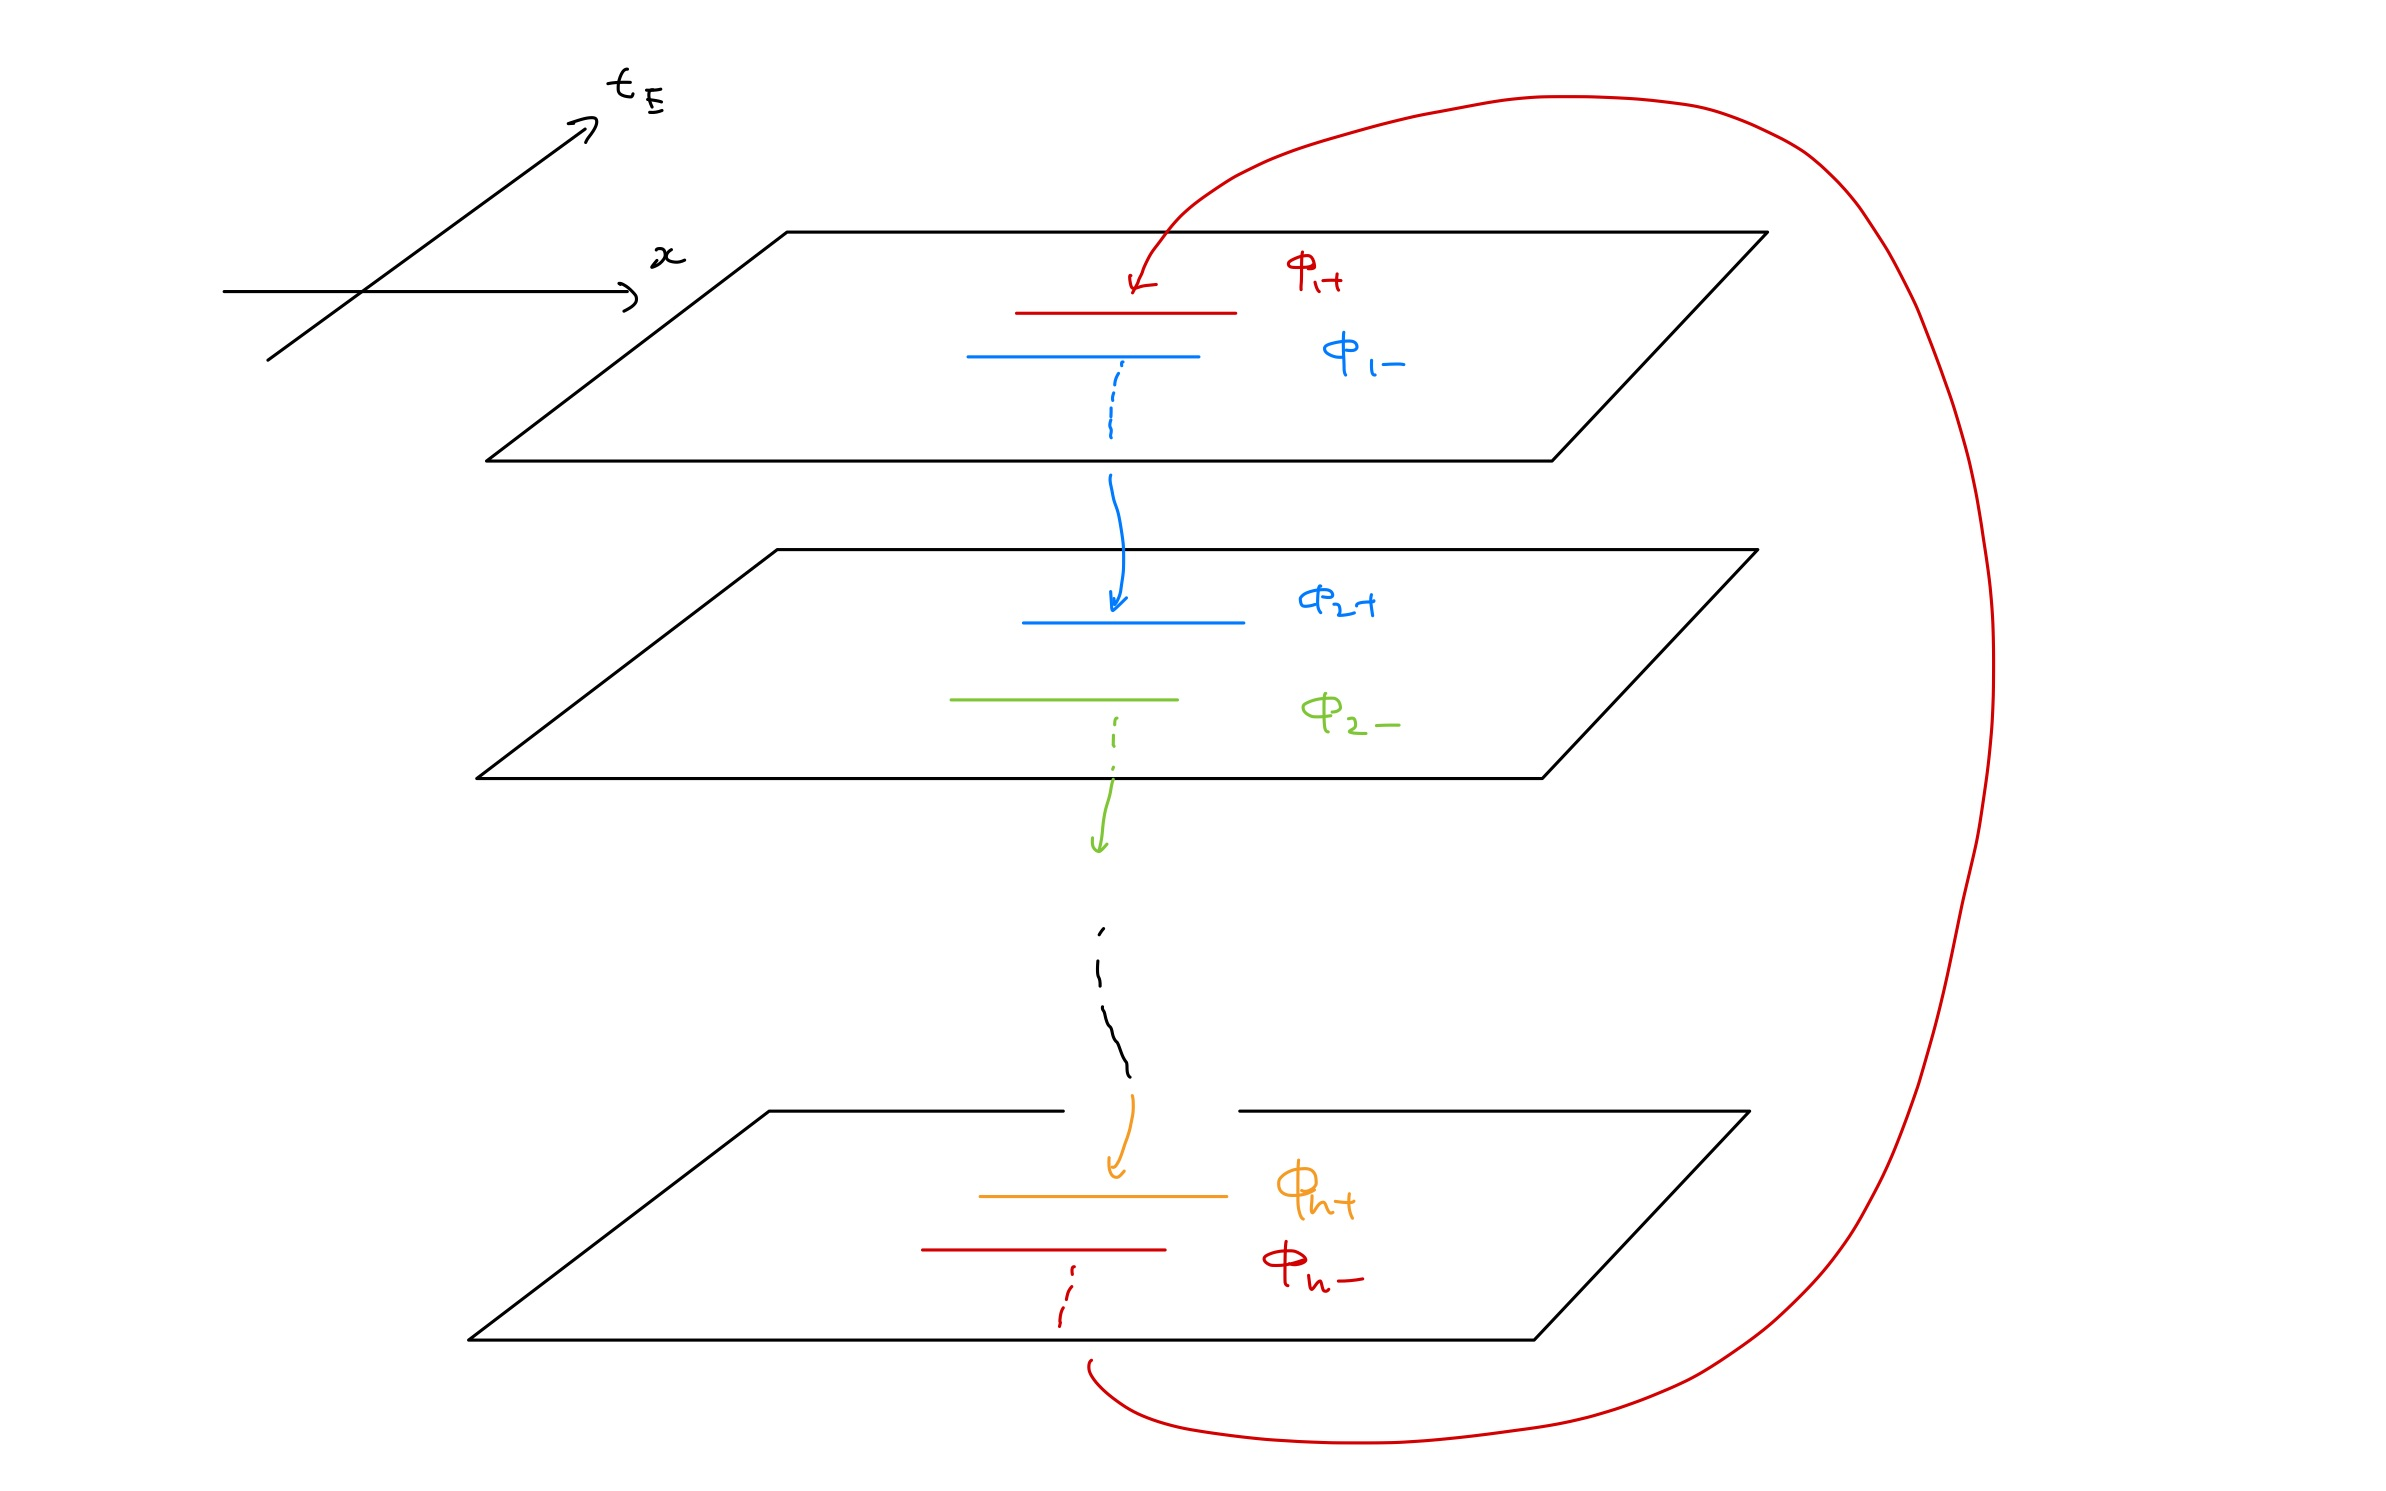
\includegraphics[keepaspectratio,width=0.8\linewidth]{fig/replica.jpg}
  \caption{$Z_{n}$の経路積分のイメージ}
\end{figure}


\subsection{ツイスト場による計算}

今考えている空間には,リーマン面の間のグローバル対称性がある.例えば,次のツイスト演算子
\begin{equation}
  \sigma_{+}^{k}\phi_{k}(\tau,x)
  =
  \phi_{k+1}
  ,\ 
  \sigma_{-}^{k}\phi_{k}(\tau,x)  
  =
  \phi_{k-1}(\tau,x)
  \label{def_twist}
\end{equation}
などもそのグローバル対称性になっている.

ここで,\eqref{sec3_1_eq1}を書き直してみると
\begin{equation}
  \tr_{A}\rho_{A}^{n}
  =
  \dfrac{\displaystyle
    \int_{\mathcal{R}^{n}}\mathcal{D}\phi\ 
    e^{-S[\phi]}
  }{\displaystyle
    \int_{\mathbb{R}^{n}}\mathcal{D}\phi\ 
    e^{-S[\phi]}
  }
\end{equation}
となるが,ここで\textbf{分子と分母の寄与の差はリーマン面のブランチカットの部分しかない}ことに気がつくであろう.この寄与の差は,先ほど定義したツイスト演算子\eqref{def_twist}の期待値で拾ってくることができる\cite{Lunin_CorrelationFunctions_2001}.すなわち
\begin{equation}  
  \tr_{A}\rho_{A}^{n}
  =
  \prod_{k=1}^{n}
  \ev*{\sigma_{+}^{k}(+0,u)\sigma_{-}^{k}(-0,v)}
\end{equation}
である\footnote{
  この関係の説明は思ったよりも長いので,ここでは参考文献\cite{Lunin_CorrelationFunctions_2001}に丸投げします.が,たぶん感覚的にはこんなところでいいはず.
}.

さて,あとはツイスト演算子の期待値を求めればよい.導出は余裕があったら書こうと思うが\footnote{
  ありませんでした!(というか,勉強が間に合いませんでした.)
}
\begin{equation}
  \ev*{\sigma_{+}^{k}(+0,u)\sigma_{-}^{k}(-0,v)}
  =
  \left( \frac{u-v}{\varepsilon} \right)^{-c(1-1/n^2)/6}  
\end{equation}
である.よって,レニーエントロピーは
\begin{equation}
  S_{n}
  =
  \frac{1}{1-n}\log\left( \frac{u-v}{\varepsilon} \right)^{-c(n-1/n)/6}
  =
  \frac{c}{6}\left( 1+\frac{1}{n} \right)\log\frac{u-v}{\varepsilon}
\end{equation}
となり,$n\rightarrow 1$の極限をとれば
\begin{equation}
  S_{A}
  =
  \frac{c}{3}\log\frac{u-v}{\varepsilon}
  \label{entropy_cft}
\end{equation}
となる.


\section{Ryu-Takayanagi公式}

さて,AdS/CFT対応というくらいなので,CFT$_2$で計算できたエントロピーも,何かしらの意味でAdS$_3$から計算できると考えるのが人情だろう.そのような対応関係は予想ではあるが実際に見つかっており,\textbf{Ryu-Takayanagi}予想\cite{Ryu_AspectsHolographic_2006}(RT公式)と言われている.この予想は完全な証明が得られているわけではないが,いくつものケースでその関係の成立が確認されている.この章では,実際に前節で用いた公式から求めたCFT$_2$でのエントロピーの結果と,AdS$_3$でのエントロピーが確かに一致していることを見ていこうと思う.

\subsection{RT公式のモチベーション}

RT公式は,ある意味で\textbf{ベッケンシュタイン・ホーキング公式}(BH公式)の一般化といわれている.BH公式は,次のブラックホールの熱力学の法則\cite{Bardeen_FourLaws_1973}
\begin{itemize}
  \item 
  事象の地平面では重力$\kappa$は一定である.(第0法則)
  \item 
  $M$を質量,$\Omega$を角速度,$\Phi$を電気的なポテンシャルとしたとき,$M$の変化は
  \begin{equation}
    \dd M
    =
    \frac{\kappa}{8\pi G}\delta A
    +
    \Omega\delta J
    +
    \Phi\delta Q
  \end{equation}
  を満たしている.ただし,$A$は面積,$J$は角運動量で$Q$は電荷.(第1法則)
  \item 
  系全体のエントロピーは減少しない.(第2法則)
  \item 
  有限回の操作では,表面の重力を0にすることはできない.(第3法則)
\end{itemize}
から導かれる\footnote{
  この法則が``熱力学の法則''と言われているのは,もちろん熱力学の法則のアナロジーである.例えば,第1法則は,ギブスの関係式
  $$
    \dd U
    =
    T\dd S
    -
    p\dd V
  $$
  によく似ている.
}.第0法則により,平衡状態の重力$\kappa$が温度のようにみなせるため
\begin{equation}
  \kappa
  \equiv
  2\pi T_{H}
\end{equation}
と$T_{H}$を定めれば,第2法則で$J=0,\ Q=0$として
\begin{equation}
  (\dd M
  =)
  \frac{1}{4G}\cdot T_{H}\delta A
\end{equation}
である.この関係は,ギブスの関係式$\dd Q=T\dd S$とみなせることから,$\dd S_{BH}\equiv \delta A/4G$という関係が成り立つと予想することができ,これは結局,次のBH公式
\begin{equation}
  S_{BH}
  =
  \frac{A}{4G}
  \label{BH_formula}
\end{equation}
に対応することになる\footnote{
  これだと,少し騙されたような気になる人がいるかもしれないが,一般相対性理論から(正確にいうとその直接的な熱力学から)導出する方法もあるらしい.例えば,Fursaevのレビュー\cite{Fursaev_BlackHole_2022}の5章とか.
}.

この関係式\eqref{BH_formula}は熱力学的な量であるエントロピーが,その``表面積''に比例していることを示唆している.これは私たちの直感に大いに反している.エントロピーは,考えている対象がどれほどの情報を保有しているかを記述しており,基本的に体積に比例して大きくなると考えられるからである.RT公式は,そういった意味でBH公式\eqref{BH_formula}の一般化となっている.次節では,その主張について見ていこう.


\subsection{主張とエントロピーの計算}

RT公式の主張は簡単に言うと次の通りである:

\begin{flushleft}
  ある$\text{AdS}$時空のスライス$\Sigma$を考える.このとき,そのスライスの部分空間$A(\subset \partial\Sigma)$の境界面が$\text{CFT}$であるとき,そのエンタングルメントエントロピーに対して次の関係
  \begin{equation}
    S_{A}
    =
    \text{min}
    \frac{\text{Area}(A)}{4G}
    \label{RT_formula}
  \end{equation}
  が成立する.
\end{flushleft}

もちろん,複雑なケースに応用するためにはもう少しこの主張を明らかに書く必要があるが,今回計算するケースでは詳細な概念を定義する必要はない.

\eqref{RT_formula}にあらわれている$\text{Area}(A)$は,領域$A$の面積であるが,エントロピーはCFTとなる境界のうち,最小の面積で与えられる.また,定数$G$は自由度換算によって決まってくる定数で,今回のケースでは
\begin{equation}
  \frac{1}{G}
  =
  \frac{3}{2}c
  \label{constant_G}
\end{equation}
である\footnote{
  今回はプランク長$l_{\text{Pl}}$やプランク定数$\hbar$を1にとっている.
}.

\begin{figure}[ht]
  \centering
  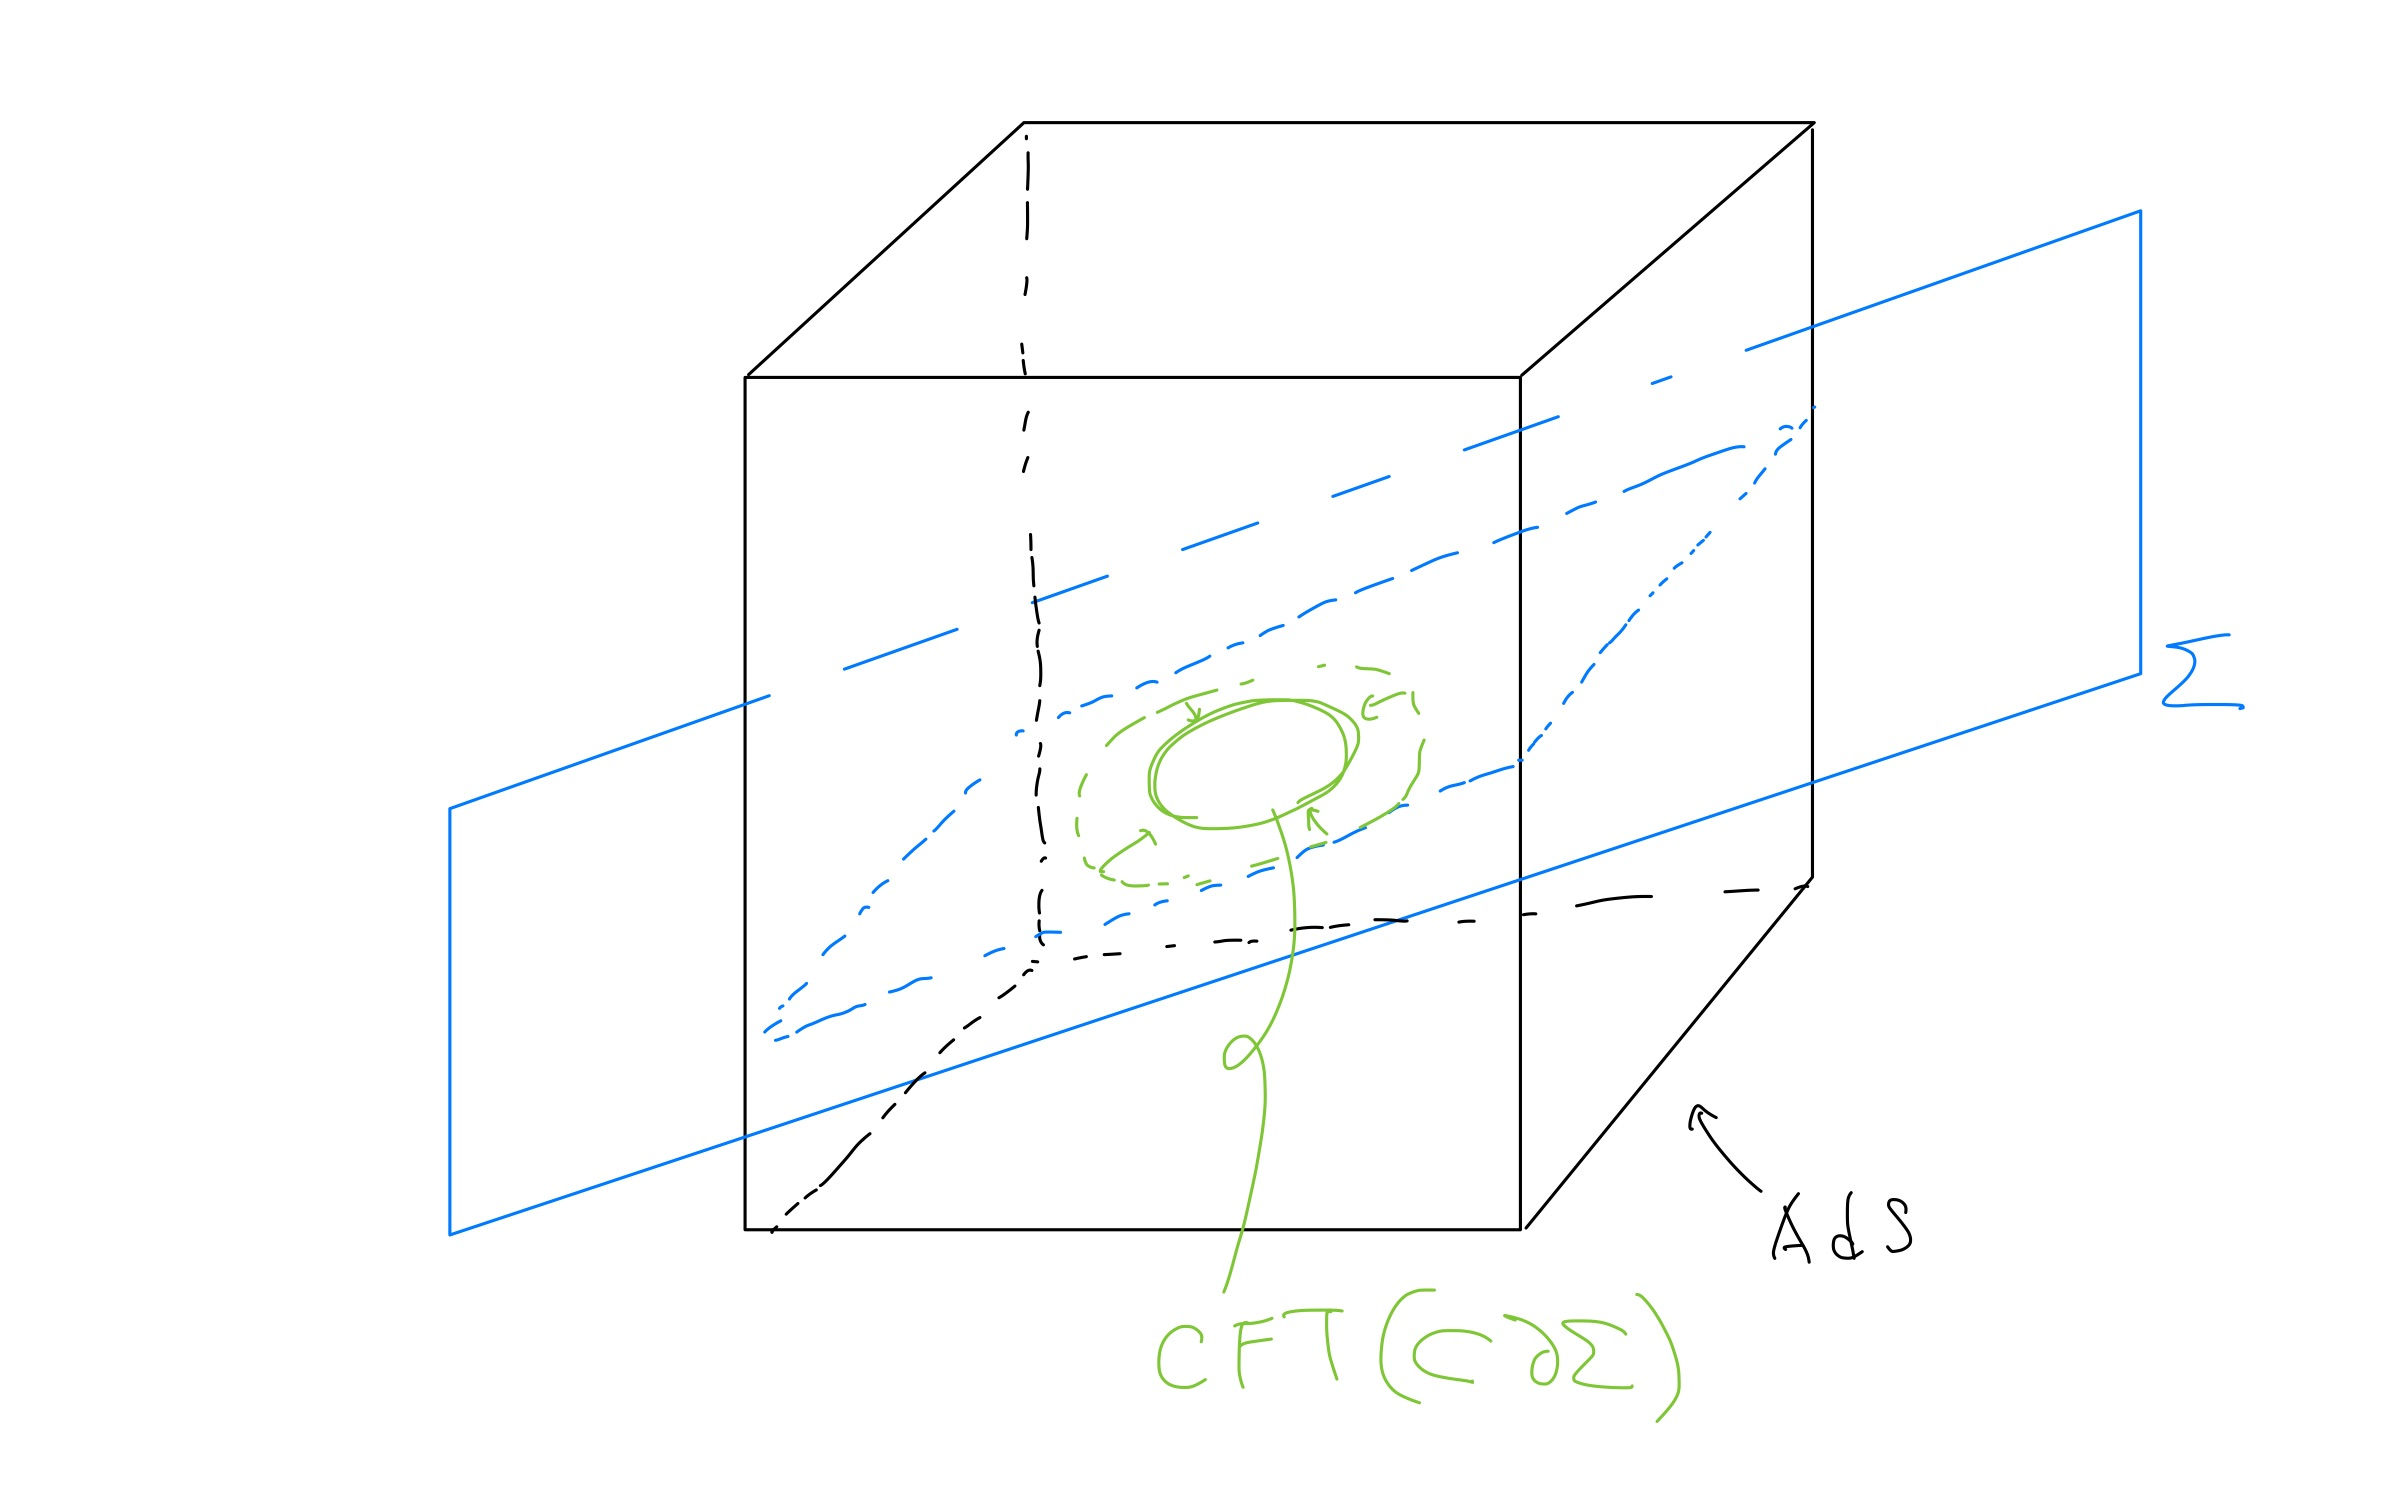
\includegraphics[keepaspectratio,width=0.8\linewidth]{fig/cft_boundary.jpg}
  \caption{スライス$\Sigma$と共形境界のイメージ}
\end{figure}

さて,今回の場合はAdS$_{3}$の計量は\eqref{AdS_metric_tzx}だとし,$t=0$のスライス$\Sigma$を考える.このとき,時空は
\begin{equation}
  \dd s^2
  =
  \frac{L^2}{z^2}(\dd x^2+\dd z^2)
\end{equation}
で書くことができる.この領域$\Sigma$での境界で面積が最小の要素というのは測地線のことなので,まずは$x_1=-l/2$と$x_2=l/2$を結ぶ測地線の長さを求めておこう.その測地線は円なので
\begin{equation}
  x(t)
  =
  \frac{l}{2}\cos t
  ,\ 
  z(t)
  =
  \frac{l}{2}\sin t
  \quad
  \left(  
    \frac{\varepsilon}{l}\leq t\leq\frac{\pi}{2}
  \right)
\end{equation}
と座標を決めておくと,測地線の長さは
\begin{equation}
  \text{Area}(A)
  =
  \int\dd s
  =
  2\int_{\varepsilon/l}^{\pi/2}
  \frac{\dd t}{\sin t}
  =
  2\log \frac{l}{\varepsilon}
\end{equation}
となる.

\begin{figure}[ht]
  \centering
  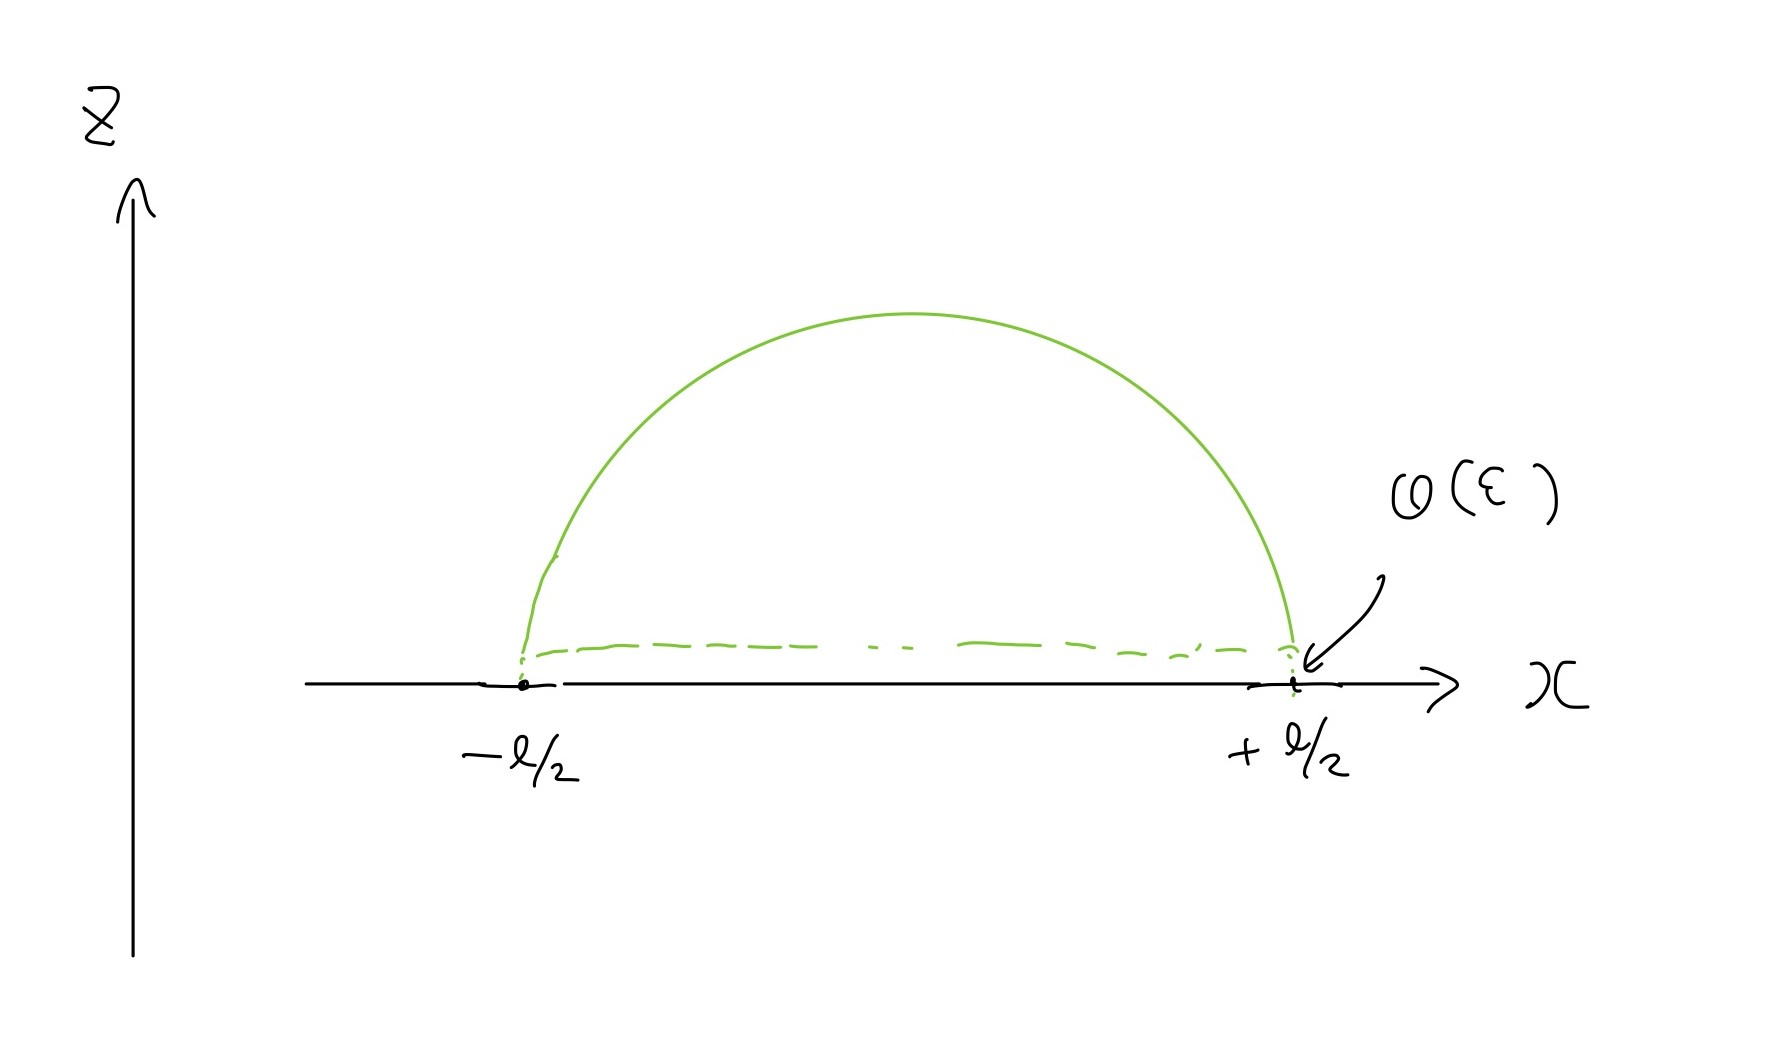
\includegraphics[keepaspectratio,width=0.8\linewidth]{fig/geodecies.jpg}
  \caption{スライス$\Sigma$での測地線}
\end{figure}

したがって,\eqref{RT_formula}と\eqref{constant_G}から,エントロピーは
\begin{equation}
  S_{A}
  =
  \frac{c}{3}\log \frac{l}{\varepsilon}
\end{equation}
となる.このエントロピーは,前章で求めた結果\eqref{entropy_cft}と一致している.


\section{あとがき}

今回はAdS/CFT対応について話してきました.一番計算が簡単なケースを書いたので,なんとなく騙された感じになった方もいるかと思います.しかしながら,このエントロピーの計算も多くの場合で対応関係があることが確かめられているそうで,非常に有力な理論であることには間違いないでしょう\footnote{
  2015年には,\href{https://breakthroughprize.org/Laureates/1/P2/Y2015}{物理学ニューホライズン賞}も授与されています.もちろん,何か賞が与えられたからと言ってその理論が正しいわけではないですが,多くの専門家がエントロピーと重力の間に密接なつながりがあるのではないかと考えているはずです.
}.実際に,さらにこの公式の適用範囲を一般化したHRT公式\cite{Hubeny_CovariantHolographic_2007}などがすぐに見つかっており,その後も色々な関係が発見されているらしいです.また,今回は,RT公式が予想であるということを強調しましたが,公式の証明はいろいろ試みがあるらしいです.それらは,Fursaevによる証明\cite{Fursaev_ProofHolographic_2006}に始まり,Casini, Huerta, Myersらによる証明\cite{Casini_DerivationHolographic_2011},Lewkowycz, Maldacenaらによる証明\cite{Lewkowycz_GeneralizedGravitational_2013}といったものがあるそうです.また,直接的な証明とは異なりますが,エンタングルメントエントロピーとして成立していてほしい性質もよく確認されているらしいですね.(subadditivityとか)

本当はこれらのこともよく勉強して,ここで書こうかと思っていたのですが,残念ながら力及ばずでした.ですので,以上の文献紹介をもってその代わりとさせていただきます.今回の内容は,「ホログラフィックエンタングルメントエントロピー」といったテーマでくくられることが多いと思うので,もし私の記事を読んで興味を持っていただいた方がいらっしゃったら,そのようなキーワードで調べていただくと色々資料が手に入るかと思います.私が今回の記事の作成にあたってよく勉強したのは\cite{Ammon_GaugeGravity_2015}, \cite{Headrick_LecturesEntanglement_2019}, \cite{Rangamani_HolographicEntanglement_2017}でした.ひとつめは,AdS/CFT対応のゲージ/重力対応的な側面で非常にスタンダードです\footnote{
  どちらかというと,私はこっちの内容のほうが興味があるので,もう少し勉強をするかもしれませんし,しないかもしれません.
}.残りの文献は,エントロピーの話が多く,特に参考になりました.また,日本語の文献では\cite{高柳_ホロ_2014}が手に入るのですが,研究室のはどこかに行きましたし,図書館のはなんか汚かったのであまり目を通していません.

先日の超対称性の記事に続き,今回の私の記事を読んでくださった皆さん,本当にありがとうございました\footnote{
  そして,なんか中途半端な内容で,すみません.
}.忘年会に出られなくてすみません.あとで,私の歌をきかせてあげたいと思います.よいお年を!


\bibliography{hoge}
\bibliographystyle{ytphys}

\end{document}
